% =============================================================================
% Rapport technique — Lecture de texte dans l'espace public pour personnes
% malvoyantes.
%
% Compilation (depuis docs/rapport/) :   latexmk -pdf rapport.tex
% Les tableaux et figures chiffrés proviennent de results/benchmark/, produits
% par scripts/benchmark.py : relancer le benchmark puis recompiler met tout le
% document à jour (y compris les chiffres cités dans le texte, via chiffres.tex).
% =============================================================================
\documentclass[11pt,a4paper]{article}

\usepackage[utf8]{inputenc}
\usepackage[T1]{fontenc}
\usepackage{lmodern}
\usepackage[french]{babel}
\usepackage[margin=2.4cm]{geometry}
\usepackage{graphicx}
\usepackage{booktabs}
\usepackage{amsmath,amssymb}
\usepackage{float}
\usepackage{caption}
\usepackage{subcaption}
\usepackage{xcolor}
\usepackage{tikz}
\usetikzlibrary{arrows.meta,positioning,shapes.geometric}
\usepackage{enumitem}
\usepackage{microtype}
\usepackage[hidelinks]{hyperref}

\graphicspath{{../figures/}{../../results/benchmark/}}
\captionsetup{font=small,labelfont=bf}
\setlist{nosep,leftmargin=*}
\emergencystretch=3em

% Chiffres générés par le benchmark (valeurs par défaut si absent)
\IfFileExists{../../results/benchmark/chiffres.tex}{% Généré par scripts/benchmark.py — ne pas modifier à la main
\newcommand{\nbImages}{50}
\newcommand{\configFinale}{etape4\_v2 : mser + otsu}
\newcommand{\baseFmed}{0{,}013}
\newcommand{\baseFmoy}{0{,}086}
\newcommand{\basePmed}{0{,}007}
\newcommand{\baseRmed}{0{,}120}
\newcommand{\baseCERmed}{6{,}59}
\newcommand{\finFmed}{0{,}281}
\newcommand{\finFmoy}{0{,}326}
\newcommand{\finFicBas}{0{,}12}
\newcommand{\finFicHaut}{0{,}41}
\newcommand{\finPmed}{0{,}250}
\newcommand{\finRmed}{0{,}400}
\newcommand{\finCERmed}{0{,}67}
\newcommand{\finMieux}{32}
\newcommand{\finEgal}{14}
\newcommand{\finPire}{4}
\newcommand{\finP}{$<$\,0{,}001}
\newcommand{\facteurF}{21}
\newcommand{\basePsmTroisFmed}{0{,}000}
}{%
  \newcommand{\nbImages}{?}\newcommand{\configFinale}{?}\newcommand{\baseFmed}{?}%
  \newcommand{\baseFmoy}{?}\newcommand{\basePmed}{?}\newcommand{\baseRmed}{?}%
  \newcommand{\baseCERmed}{?}\newcommand{\finFmed}{?}\newcommand{\finFmoy}{?}%
  \newcommand{\finFicBas}{?}\newcommand{\finFicHaut}{?}\newcommand{\finPmed}{?}%
  \newcommand{\finRmed}{?}\newcommand{\finCERmed}{?}\newcommand{\finMieux}{?}%
  \newcommand{\finEgal}{?}\newcommand{\finPire}{?}\newcommand{\finP}{?}\newcommand{\facteurF}{?}}

\newcommand{\tableauOuNote}[2]{\IfFileExists{../../results/benchmark/#1}{\input{../../results/benchmark/#1}}%
  {\begin{center}\fbox{\parbox{0.9\linewidth}{\small\textit{#2}}}\end{center}}}
\newcommand{\fichier}[1]{\texttt{#1}}

\title{\textbf{Assistance à la lecture d'informations dans l'espace public\\pour les personnes malvoyantes}\\[0.4em]
\large Rapport technique — détection et reconnaissance de texte dans des scènes urbaines}
\author{Zitouni Zaid, Zerrif Haitam, Zbayar Ziad}
\date{Novembre 2026}

\begin{document}
\maketitle

\begin{abstract}
Ce projet développe une chaîne de traitement qui extrait automatiquement le texte présent sur une photographie prise dans l'espace public (plaques de rue, panneaux, numéros, enseignes) et le restitue sous une forme lisible par une personne malvoyante. Elle repose uniquement sur des techniques classiques de traitement d'images (filtrage, histogrammes, binarisation, morphologie mathématique, régions extrémales stables) mises en œuvre avec Python, OpenCV, NumPy et SciPy, et sur le moteur de reconnaissance Tesseract.
Sur une base de \nbImages{} photographies annotées, appliquer Tesseract directement à l'image (baseline) ne donne presque rien d'exploitable : F1 médian des mots de \baseFmed{}, précision médiane de \basePmed{}. Le diagnostic montre que le défaut principal n'est ni le bruit ni le contraste, mais la \emph{scène} : Tesseract invente des lettres dans les arbres et les façades. Localiser d'abord le texte, puis lire chaque zone séparément, porte le F1 médian à \finFmed{} (IC à 95\,\%~: [\finFicBas\,; \finFicHaut]) avec la configuration finale (détection MSER, binarisation d'Otsu et lecture zone par zone), une amélioration significative (\finMieux{} images améliorées, \finPire{} dégradées, test de Wilcoxon $p$~\finP{}). Les limites restantes (écriture arabe, lettres gravées, néons, texte minuscule) sont analysées une à une.
\end{abstract}

\tableofcontents
\newpage

% -----------------------------------------------------------------------------
\section{Introduction}
% -----------------------------------------------------------------------------

\subsection{Contexte et problématique}
Pour une personne malvoyante, s'orienter en ville suppose de lire des informations conçues pour être vues : nom de la rue, numéro de l'immeuble, direction indiquée par un panneau, nom d'un commerce. Un smartphone peut photographier la scène ; il reste à en extraire le texte et à le restituer sous une forme accessible.

La reconnaissance optique de caractères (OCR) est une technologie mûre pour les documents numérisés : page blanche, texte noir, lignes horizontales, éclairage uniforme. Une photographie de rue ne présente aucune de ces propriétés : le texte n'occupe qu'une petite partie de l'image, il est entouré d'éléments très texturés (feuillage, briques, véhicules), l'éclairage est inégal (ombres portées, contre-jour, nuit), la polarité varie (lettres blanches sur fond bleu, noires sur fond blanc), les polices sont variées et la perspective déforme les lignes.

\subsection{Objectifs}
Le cahier des charges fixe quatre objectifs : améliorer la lisibilité des images (débruitage, contraste), détecter les zones contenant du texte, extraire les caractères et les mots par OCR, et restituer le texte à l'utilisateur. Il impose les outils (Python, OpenCV, NumPy, SciPy, Matplotlib, Tesseract) et demande de comparer les méthodes utilisées.

\subsection{Démarche et contributions}
Plutôt que d'assembler un pipeline d'un bloc, nous avons mesuré l'apport de chaque étape par rapport à un point de départ explicite (la baseline) et avec les mêmes métriques. Cette démarche a conduit à un résultat parfois contre-intuitif : sur l'image entière, ni le débruitage ni la binarisation ne changent l'ordre de grandeur des performances ; c'est la localisation du texte qui est décisive. Les contributions sont :
\begin{itemize}
\item une base de \nbImages{} photographies urbaines sous licence libre, annotées selon une règle explicite ;
\item un pipeline modulaire et reproductible (environnement figé avec \texttt{uv}, image Docker) ;
\item un protocole d'évaluation adapté aux scènes (précision et rappel des mots, intervalles de confiance, tests appariés) ;
\item une analyse détaillée des échecs, qui sépare les erreurs de localisation de celles de reconnaissance.
\end{itemize}

% -----------------------------------------------------------------------------
\section{Données}
% -----------------------------------------------------------------------------

\subsection{Constitution de la base}
Les images proviennent de Wikimedia Commons, choisi pour trois raisons : accès sans compte ni clé d'API, licence explicite pour chaque fichier, et catégories thématiques (plaques de rue, numéros de maisons, signalisation). Le script \fichier{scripts/telecharger\_commons.py} interroge l'API de Commons, ne conserve que les licences réutilisables (CC0, domaine public, CC~BY, CC~BY-SA ; les clauses NC et ND sont exclues car nos traitements modifient les images) et enregistre pour chaque fichier l'auteur, la licence et la page source dans \fichier{data/SOURCES.csv}, ce qu'exigent les licences CC~BY et CC~BY-SA. Les images sont téléchargées en 1\,600 à 1\,920~px de large.

Après tri manuel, la base compte \nbImages{} images réparties en quatre catégories (tableau~\ref{tab:base}). Elle mêle des scènes françaises et marocaines, y compris de la signalisation bilingue français--arabe.

\begin{table}[htbp]
\centering\small
\begin{tabular}{lrl}
\toprule
Catégorie & Images & Exemples \\
\midrule
plaques & 35 & plaques de rue émaillées ou gravées, plaques commémoratives \\
panneaux & 7 & panneaux directionnels, signalisation routière \\
affiches & 5 & enseignes de commerces, affiches \\
numeros & 3 & numéros de bâtiments \\
\midrule
total & 50 & \\
\bottomrule
\end{tabular}
\caption{Composition de la base de test.}
\label{tab:base}
\end{table}

\subsection{Annotation}
Chaque image est accompagnée d'un fichier \fichier{data/ground\_truth/<image>.txt} contenant le texte exact visible, une ligne par ligne de texte. La règle retenue est d'annoter \emph{tout texte de signalétique lisible à l'œil nu sur l'image} (plaques, panneaux, enseignes), en respectant la casse, les accents et la ponctuation affichés, et d'exclure les plaques d'immatriculation et le texte des véhicules. Cette règle a un effet direct sur les scores : un texte lisible mais non annoté, que le système lit correctement, est compté comme une erreur. Les premières annotations ont été corrigées en ce sens (par exemple un zéro saisi à la place de la lettre \og d\fg{} de \og Clermont-Fd\fg{}, des accents omis sur \og CONTRÔLES FRÉQUENTS\fg).

\subsection{Limites de la base}
Avec \nbImages{} images, et seulement 3 à 7 dans certaines catégories, les résultats par catégorie sont indicatifs. Les plaques de rue dominent (70\,\%). Nous en tenons compte en rapportant des intervalles de confiance et en évitant de conclure sur les petites catégories. Enfin, huit vérités terrain contiennent du texte en arabe (plaques bilingues marocaines), alors que l'OCR est configuré pour le français et l'anglais : ces mots sont toujours comptés comme manqués, ce qui abaisse le rappel. Ce choix est délibéré, car il mesure la limite réelle du système dans le contexte marocain.

% -----------------------------------------------------------------------------
\section{Architecture du système}
% -----------------------------------------------------------------------------

Le système est un pipeline de six modules indépendants (figure~\ref{fig:pipeline}), chacun dans un fichier de \fichier{src/}. Chaque module expose un \emph{registre} de méthodes interchangeables désignées par leur nom (par exemple \texttt{"nlm"}, \texttt{"clahe"}, \texttt{"sauvola"}, \texttt{"mser"}), ce qui permet aux scripts de comparaison de \fichier{scripts/} d'essayer toutes les combinaisons sans modifier le code.

\begin{figure}[htbp]
\centering
\begin{tikzpicture}[
  bloc/.style={draw, rounded corners=3pt, minimum width=2.25cm, minimum height=1.25cm, align=center, font=\small, fill=#1},
  bloc/.default=gray!8,
  fleche/.style={-{Stealth[length=2.2mm]}, thick}]
\node[bloc] (a) {1. Acquisition\\\scriptsize gris, 1600 px};
\node[bloc=blue!8, right=0.45cm of a] (p) {2. Prétraitement\\\scriptsize débruitage,\\\scriptsize contraste};
\node[bloc=green!10, right=0.45cm of p] (l) {4. Localisation\\\scriptsize MSER,\\\scriptsize morphologie};
\node[bloc=green!10, right=0.45cm of l] (o) {3+5. Binarisation\\\scriptsize + OCR\\\scriptsize par région};
\node[bloc, right=0.45cm of o] (r) {6. Restitution\\\scriptsize texte, carte\\\scriptsize de lecture};
\node[bloc=red!8, below=0.9cm of o] (e) {7. Évaluation\\\scriptsize CER, WER, P/R/F1};
\draw[fleche] (a) -- (p); \draw[fleche] (p) -- (l); \draw[fleche] (l) -- (o); \draw[fleche] (o) -- (r);
\draw[fleche, dashed] (o) -- (e);
\end{tikzpicture}
\caption{Architecture du pipeline. Les numéros renvoient aux étapes du cahier des charges. Dans la configuration finale, la binarisation et l'OCR sont appliqués à chaque zone localisée et non à l'image entière (section~\ref{sec:resultats}).}
\label{fig:pipeline}
\end{figure}

\paragraph{Correspondance modules / fichiers.}
\fichier{acquisition.py} (étape 1), \fichier{preprocessing.py} (2), \fichier{binarization.py} (3), \fichier{text\_detection.py} (4), \fichier{ocr.py} (5), \fichier{restitution.py} (6), \fichier{evaluation.py} et \fichier{metrics\_image.py} (7), \fichier{visualization.py} (figures). L'application finale est \fichier{scripts/lire\_image.py}.

\paragraph{Reproductibilité.}
Les versions exactes des bibliothèques sont figées dans \fichier{uv.lock} (gestionnaire \texttt{uv}, Python 3.14). Une image Docker inclut en plus Tesseract et ses données de langue (français, anglais, arabe), seule dépendance non Python. OpenCV est volontairement limité à la version~4 : dans OpenCV~5.0.0, le détecteur MSER ne renvoie aucune région, même sur un texte parfaitement net (0 région contre 11 avec OpenCV~4.14 sur la même image de test). Ce défaut, découvert pendant le projet, aurait faussé toute la comparaison des détecteurs.

% -----------------------------------------------------------------------------
\section{Méthodes}
% -----------------------------------------------------------------------------

\subsection{Acquisition}
L'image est lue (avec \texttt{np.fromfile} et \texttt{cv2.imdecode}, qui gèrent les chemins accentués sous Windows), convertie en niveaux de gris et redimensionnée pour que son plus grand côté mesure 1\,600~px (interpolation par moyenne de zone pour la réduction). Cette normalisation rend les paramètres exprimés en pixels (taille des filtres, des tuiles, des éléments structurants) comparables d'une image à l'autre.

\subsection{Prétraitement}

\paragraph{Estimation du bruit.} Pour adapter la force du débruitage, l'écart-type du bruit est estimé par la méthode d'Immerkær~\cite{immerkaer}, qui convolue l'image avec un masque annulant les zones lisses et les rampes :
\[
\hat\sigma = \sqrt{\frac{\pi}{2}}\,\frac{1}{6(W-2)(H-2)}\sum_{x,y}\bigl|(I * M)(x,y)\bigr|,\qquad
M=\begin{pmatrix}1&-2&1\\-2&4&-2\\1&-2&1\end{pmatrix}.
\]

\paragraph{Débruitage.} Quatre filtres sont comparés :
\begin{itemize}
\item \textbf{gaussien} : référence ; il lisse le bruit mais aussi les bords des lettres ;
\item \textbf{médian} ($3\times3$) : adapté au bruit impulsionnel (poussière, pixels morts) et préserve assez bien les contours ;
\item \textbf{bilatéral}~\cite{bilateral} : moyenne pondérée à la fois par la distance spatiale et par l'écart d'intensité, ce qui lisse les zones homogènes sans traverser les bords ;
\item \textbf{moyennes non locales} (NLM)~\cite{nlm} : chaque pixel est remplacé par une moyenne de pixels dont le \emph{voisinage} ressemble au sien, recherchés dans une fenêtre de $21\times21$ ; la force $h$ est fixée à $1{,}2\,\hat\sigma$ pour ne pas sur-lisser une image déjà propre.
\end{itemize}

\paragraph{Contraste.} L'égalisation globale d'histogramme étale l'histogramme cumulé sur $[0,255]$ ; elle sature les zones claires quand l'éclairage n'est pas uniforme. \textbf{CLAHE}~\cite{clahe} égalise par tuiles ($8\times8$, soit environ 200~px, la taille d'une plaque) en limitant la pente de la transformation (\emph{clip limit} de 2), ce qui évite d'amplifier le bruit. Nous testons aussi une correction gamma automatique ($\gamma = \ln 0{,}5 / \ln \bar I$, qui ramène la moyenne vers 128) et un étirement linéaire entre les centiles 2 et 98.

\paragraph{Validation sur bruit contrôlé.} Pour juger les filtres indépendamment de l'OCR, une image propre (bruit estimé $\hat\sigma \le 6$) sert de référence ; on y ajoute un bruit connu puis on mesure le SSIM~\cite{ssim} entre la référence et l'image filtrée. Sur les 44 images de la base assez propres pour servir de référence, NLM est le meilleur filtre contre un bruit gaussien de $\sigma=15$ (SSIM moyen de 0,81, contre 0,48 sans filtre, 0,80 pour le bilatéral et 0,78 pour le flou gaussien), et le médian contre un bruit impulsionnel de 5\,\% (0,89, contre 0,61 pour NLM et 0,35 pour le bilatéral, qui préserve les points parasites comme des bords), conformément à la théorie. NLM est en revanche coûteux : environ 1,1~s par image, contre 46~ms pour le bilatéral. La figure~\ref{fig:debruitage} montre l'effet sur des lettres gravées. Une référence bruitée pénaliserait à tort un bon filtre, qui retirerait aussi le bruit d'origine : c'est pourquoi seules les images déjà propres servent de référence.

\begin{figure}[htbp]
\centering
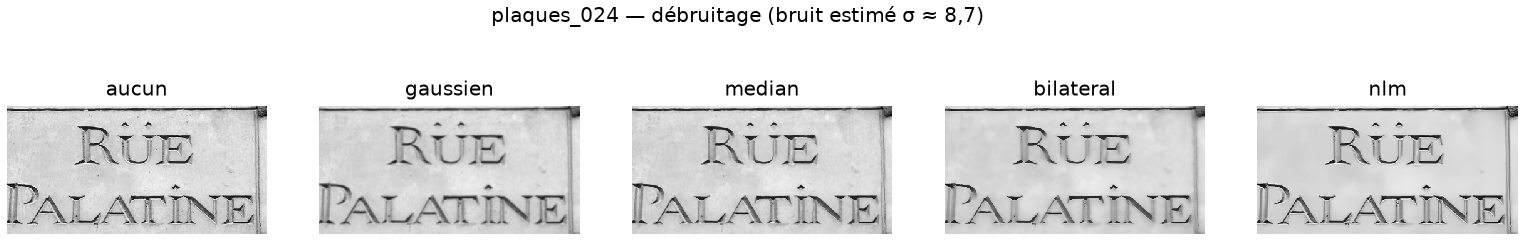
\includegraphics[width=\linewidth]{debruitage_zoom_024.png}
\caption{Plaque gravée (plaques\_024, bruit estimé $\hat\sigma \approx 8{,}7$) après chaque débruitage. Le flou gaussien empâte les arêtes des lettres ; le bilatéral et surtout NLM lissent le grain du marbre en conservant les arêtes.}
\label{fig:debruitage}
\end{figure}

\subsection{Binarisation}\label{sec:binarisation}
La binarisation classe chaque pixel en texte (noir) ou fond (blanc) en le comparant à un seuil $T$, global ou local.

\paragraph{Méthodes globales.} Le \textbf{seuil fixe} ($T=127$) sert de référence naïve. La méthode d'\textbf{Otsu}~\cite{otsu} choisit le seuil qui maximise la variance inter-classes
\[ T^\ast = \arg\max_T\; \omega_0(T)\,\omega_1(T)\,\bigl(\mu_0(T)-\mu_1(T)\bigr)^2, \]
où $\omega_i$ et $\mu_i$ sont les proportions et moyennes des deux classes ; elle est optimale quand l'histogramme est bimodal. La méthode du \textbf{triangle}~\cite{triangle} place le seuil au pied du pic principal ; elle convient quand le texte est très minoritaire. La figure~\ref{fig:histo} montre pourquoi un seuil unique échoue en présence d'une ombre portée : l'histogramme est bien bimodal, mais ses deux modes correspondent à l'\emph{ombre} et à la \emph{lumière}, et non au texte et au fond. Le seuil d'Otsu sépare donc la zone ombrée du reste, pas les lettres de la plaque.

\paragraph{Méthodes adaptatives.} Le seuil est calculé sur une fenêtre $w\times w$ centrée sur chaque pixel, à partir de la moyenne $m$ et de l'écart-type $s$ locaux (calculés avec des filtres moyenneurs séparables de SciPy, $s^2 = \overline{I^2} - \bar I^2$) :
\begin{align*}
\text{moyenne} - C &: T = m - C, \\
\text{Niblack~\cite{niblack}} &: T = m + k\,s,\quad k=-0{,}2, \\
\text{Sauvola~\cite{sauvola}} &: T = m\left(1 + k\left(\tfrac{s}{R}-1\right)\right),\quad k=0{,}5,\; R=128.
\end{align*}
Niblack transforme le grain d'un fond uniforme en faux texte, car quand $s$ est faible, $T \approx m$. Sauvola corrige ce défaut : quand $s \ll R$, le seuil descend nettement sous la moyenne et le fond reste blanc. La taille de fenêtre doit couvrir un caractère et un peu de fond ; nous prenons $w \approx 1{,}8$ fois la hauteur des caractères, soit 51~px sur l'image entière et une valeur déduite de la hauteur de la zone pour l'OCR par région.

\paragraph{Polarité.} Ces formules supposent un texte foncé sur fond clair, alors que beaucoup de plaques portent des lettres blanches sur fond bleu. Une première heuristique (couleur majoritaire sur les bords de l'image) se trompait sur les photos entières, dont le bord montre le mur et non la plaque. La règle retenue repose sur une propriété du texte : après une binarisation d'Otsu de la zone la plus texturée, \emph{la classe qui forme le plus d'objets de taille \og caractère\fg{} est le texte}. Elle donne la bonne polarité dans les six cas testés (trois photos entières et trois plaques recadrées).

\paragraph{Nettoyage morphologique.} Une ouverture $2\times2$ et un filtrage des composantes connexes par aire retirent les points isolés. Surtout, on supprime les composantes \emph{creuses et étendues} (boîte englobante supérieure à 20\,\% de l'image, remplissage inférieur à 15\,\%) et les \emph{longs traits} (allongement supérieur à 15) : les méthodes adaptatives font ressortir le cadre des plaques, et Tesseract, voyant le texte \og dans une case\fg, le prend pour un tableau et ne renvoie rien. Sur nos images de test synthétiques, ce seul nettoyage a fait passer les méthodes adaptatives d'un texte vide à une lecture exacte.

\begin{figure}[htbp]
\centering
\begin{subfigure}{0.62\linewidth}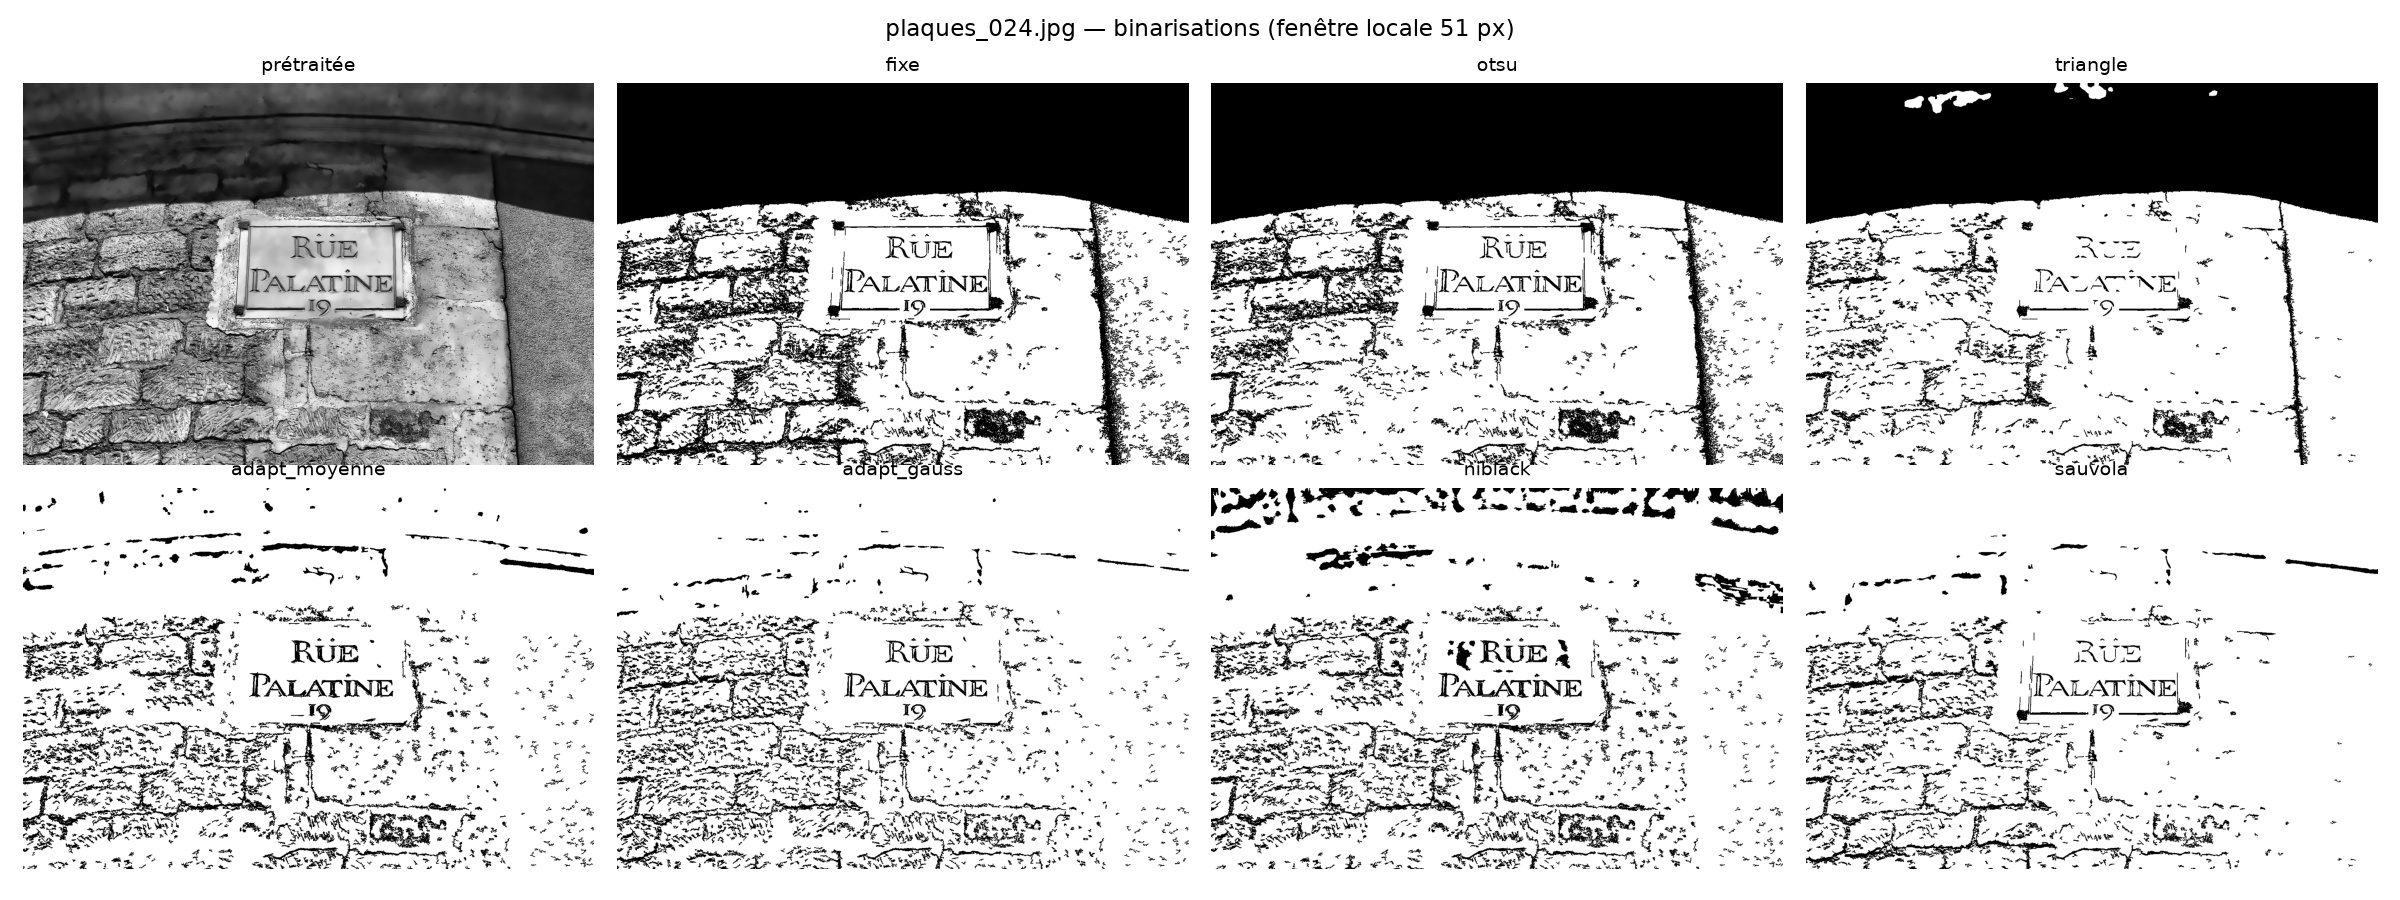
\includegraphics[width=\linewidth]{binarisation_024.png}\end{subfigure}\hfill
\begin{subfigure}{0.36\linewidth}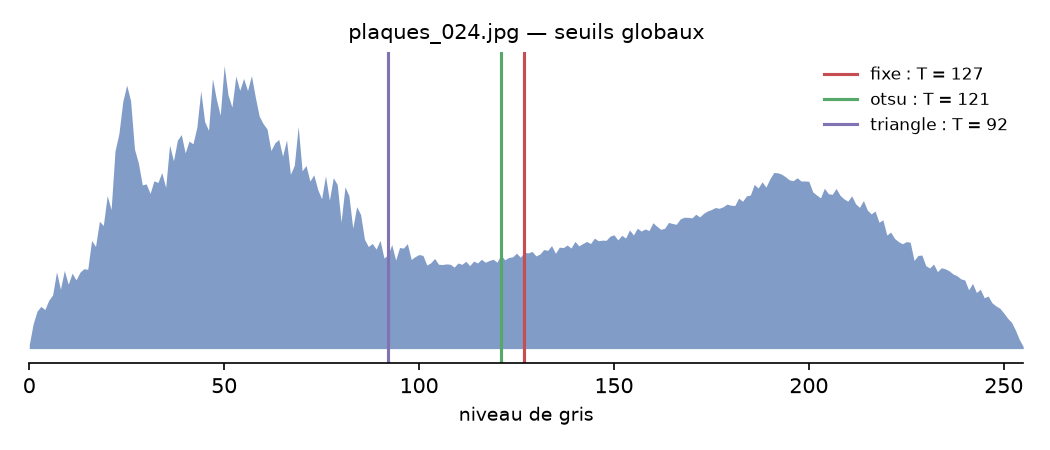
\includegraphics[width=\linewidth]{histogramme_024.png}\end{subfigure}
\caption{Plaque sous une ombre portée (plaques\_024), après NLM et CLAHE. Gauche : les seuils globaux (fixe, Otsu) noircissent toute la bande d'ombre ; les méthodes adaptatives effacent l'ombre mais transforment la maçonnerie en traits noirs, que Tesseract lit comme des lettres. Droite : les deux modes de l'histogramme sont l'ombre et la lumière.}
\label{fig:histo}
\end{figure}

\subsection{Localisation du texte}\label{sec:localisation}
Deux détecteurs sont comparés ; tous deux produisent des boîtes candidates, une par ligne de texte, ensuite vérifiées par une étape commune.

\paragraph{Contours et morphologie mathématique.} On calcule le gradient morphologique (dilatation moins érosion avec un élément $3\times3$), fort sur les bords des lettres, puis on le binarise par Otsu. Les longs traits horizontaux (bords de panneaux, corniches) sont extraits par une ouverture avec un segment de 4\,\% de la largeur, puis soustraits : sans ce retrait, la fermeture suivante soude les lettres au cadre du panneau. Une \textbf{fermeture} avec un élément horizontal (2\,\% de la largeur $\times$ 3~px) relie les lettres d'une même ligne sans relier deux lignes superposées. Les contours externes donnent les candidats, filtrés par hauteur, rapport largeur/hauteur et taux de remplissage.

\paragraph{MSER.} Une lettre est une région homogène nettement séparée de son fond : quand on fait varier le seuil, sa forme reste stable. Les régions extrémales maximalement stables (MSER)~\cite{mser} sont exactement ces régions, quelle que soit la polarité. Après un lissage bilatéral (sans lequel le bruit rend les régions instables), on garde les régions de forme compatible avec une lettre, puis on les regroupe en lignes par union-find : deux lettres sont liées si leurs hauteurs sont proches (rapport inférieur à 1,5), leurs centres alignés et leur écart horizontal inférieur à 1,2 fois leur hauteur. Cette approche par composantes connexes suit l'esprit de~\cite{neumann}.

\paragraph{Pyramide d'échelles.} Les noyaux ont une taille fixe en pixels, adaptée à des lettres de 10 à 30~px. Les grandes plaques photographiées de près (lettres de 70~px) se fragmentaient en bandes horizontales. On relance donc la détection sur l'image réduite de moitié puis au quart et on ramène les boîtes à l'échelle d'origine.

\paragraph{Vérification par segmentation des caractères.} Les deux détecteurs trouvent aussi du feuillage, des grilles ou des fenêtres. Chaque candidat est binarisé (Otsu, polarité automatique) et découpé en composantes connexes ; il n'est gardé que s'il contient au moins deux composantes de taille \og caractère\fg{} de hauteurs comparables (écart inférieur à 30\,\% de la médiane) et alignées (écart-type des lignes de base inférieur à 25\,\% de la hauteur). Le feuillage produit des composantes de toutes tailles, mal alignées. Si la vérification échoue, un \textbf{profil de projection horizontal} des composantes-caractères tente de séparer deux lignes collées (cas \og RANDAN / BRUGHEAS\fg).

\paragraph{Canaux supplémentaires (option).} La conversion en gris ne conserve que la luminance : un texte qui ne se distingue de son fond que par la couleur y devient invisible (figure~\ref{fig:couleur}). En option, la détection est aussi menée sur le canal $b$ de l'espace Lab (axe jaune--bleu) et sur l'image égalisée par CLAHE ; chaque zone est ensuite lue dans le canal où elle se détache le mieux de son fond, mesuré par le critère de séparabilité d'Otsu $\eta = \sigma_B^2/\sigma_T^2$.

\begin{figure}[htbp]
\centering
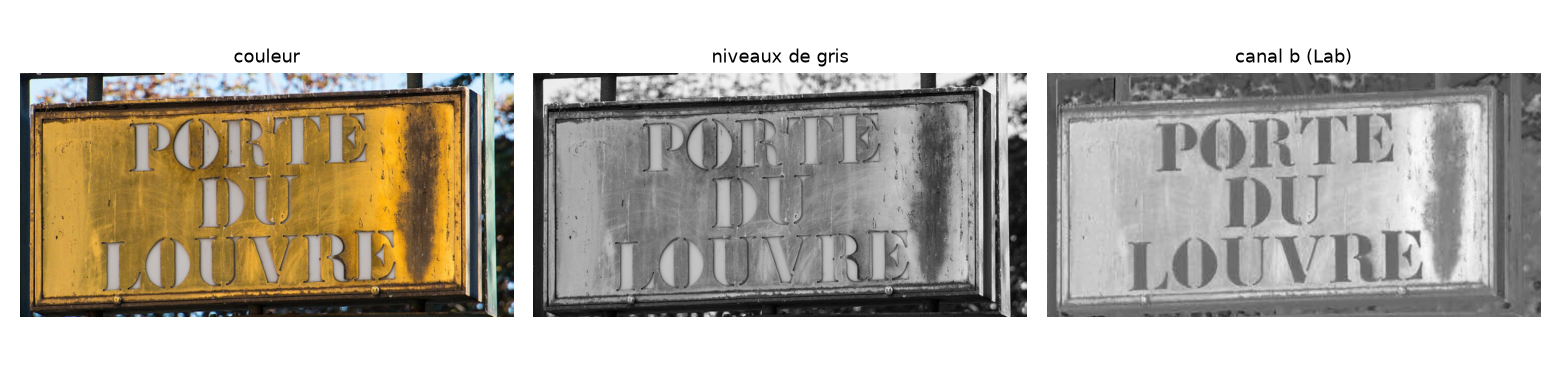
\includegraphics[width=\linewidth]{canal_couleur_016.png}
\caption{Lettres blanches sur plaque dorée : presque invisibles en niveaux de gris, nettement contrastées dans le canal $b$ de Lab.}
\label{fig:couleur}
\end{figure}

\subsection{Reconnaissance par région}
Chaque zone retenue est recadrée avec une marge de 25\,\% de sa hauteur, redimensionnée pour que la ligne mesure 48~px (Tesseract reconnaît le mieux des caractères de 30 à 40~px~\cite{tesseract}), binarisée seule, puis nettoyée de tout objet qui \emph{touche le bord} de la zone (cadre, flèche, poteau) : grâce à la marge, une vraie lettre ne touche jamais le bord. Tesseract est appelé en mode \og une ligne\fg{} (\texttt{--psm 7}, langues \texttt{fra+eng}). La fonction \texttt{image\_to\_data} fournit une confiance par mot ; seuls les mots de confiance au moins égale à 50 et contenant un caractère alphanumérique sont conservés. La figure~\ref{fig:regions} montre les zones telles que Tesseract les reçoit.

\begin{figure}[htbp]
\centering
\begin{subfigure}{0.6\linewidth}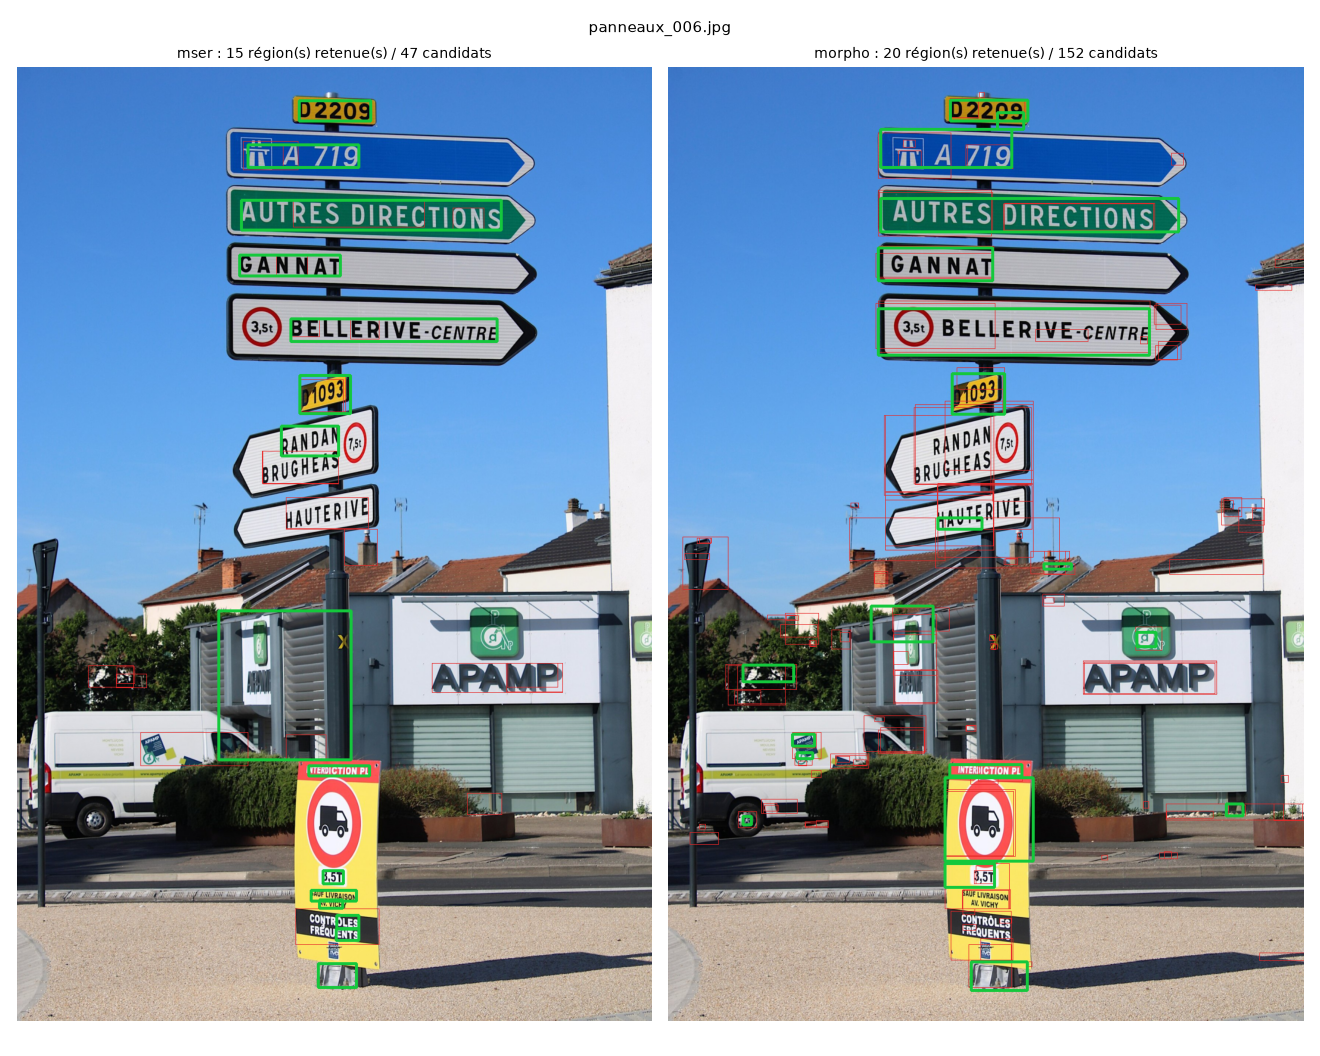
\includegraphics[width=\linewidth]{detection_006.png}\caption{Détection : morphologie (gauche), MSER (droite). Rouge fin : candidats rejetés ; vert : zones retenues.}\end{subfigure}\hfill
\begin{subfigure}{0.36\linewidth}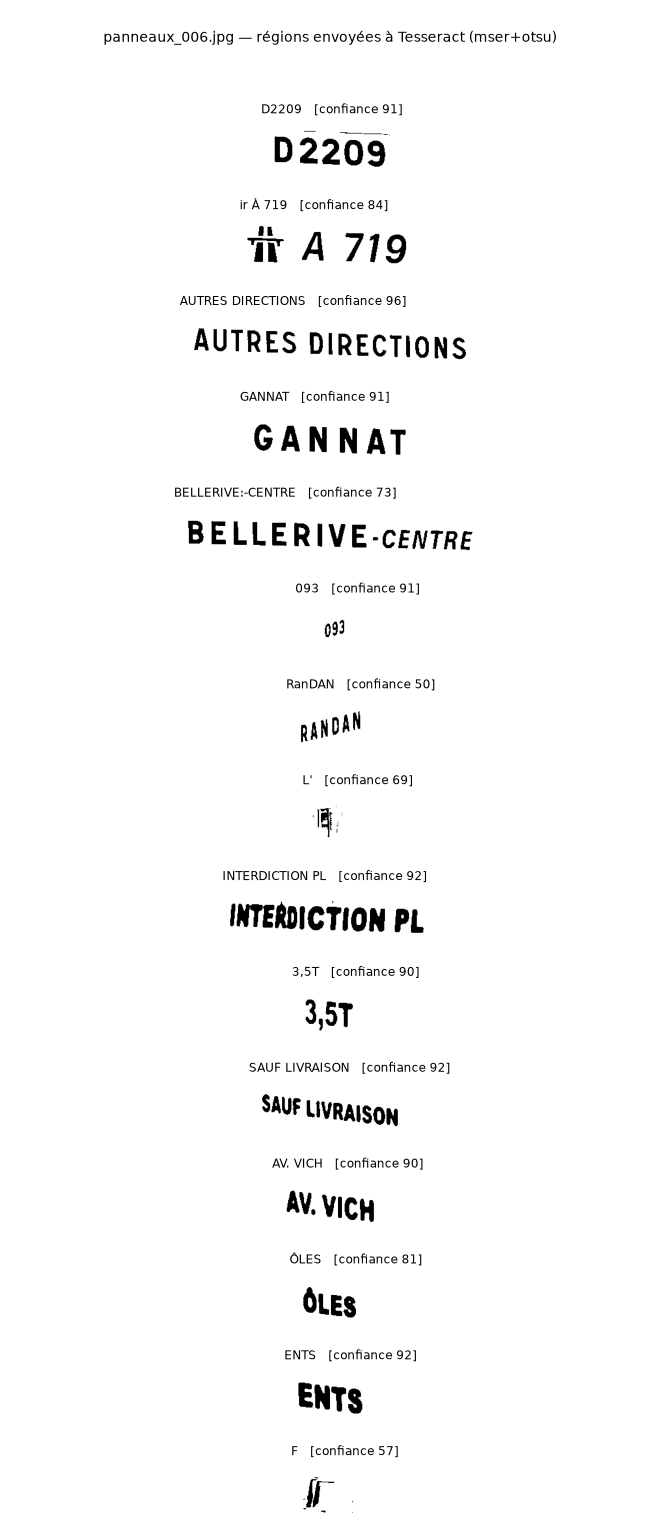
\includegraphics[width=\linewidth,height=9.5cm,keepaspectratio]{regions_006.png}\caption{Zones envoyées à Tesseract, texte lu et confiance.}\end{subfigure}
\caption{Localisation et lecture par région sur un poteau de signalisation.}
\label{fig:regions}
\end{figure}

\subsection{Restitution}
Le texte lu est nettoyé (suppression des fragments d'une ou deux lettres sans chiffre, souvent issus de pictogrammes, et des lignes répétées), puis restitué de trois façons : texte brut (exploitable par un lecteur d'écran ou une synthèse vocale), affichage console à raison d'une information par ligne, et \emph{carte de lecture} (figure~\ref{fig:carte}). Celle-ci suit les recommandations d'accessibilité pour la basse vision (WCAG~2.x, critères 1.4.3 et 1.4.6) : très grand corps, police sans empattement, jaune sur noir (rapport de contraste d'environ 17:1, au-delà du seuil de 7:1 du niveau AAA) ; la photo, avec les zones numérotées, permet à un accompagnant de vérifier l'origine de chaque ligne.

\begin{figure}[htbp]
\centering
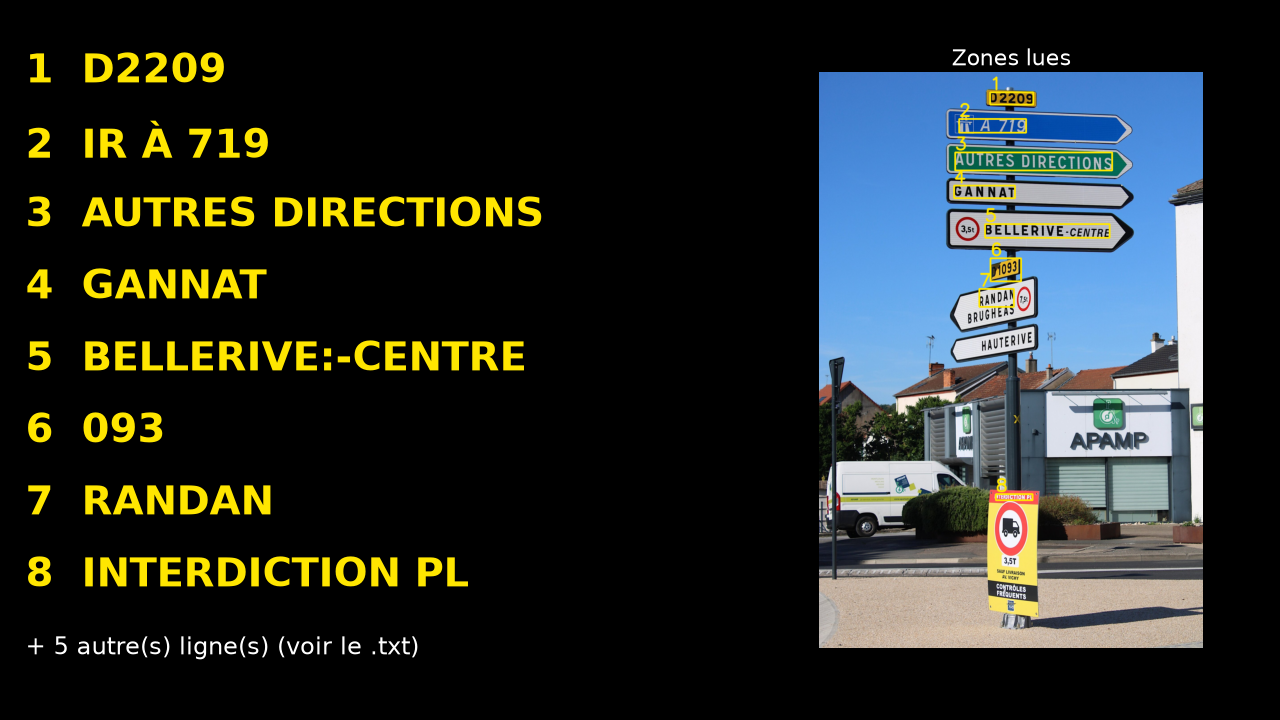
\includegraphics[width=0.85\linewidth]{carte_006.png}
\caption{Carte de lecture produite par \fichier{scripts/lire\_image.py}. Le numéro de chaque ligne est celui de sa zone sur la photo.}
\label{fig:carte}
\end{figure}

% -----------------------------------------------------------------------------
\section{Protocole d'évaluation}
% -----------------------------------------------------------------------------

\subsection{Métriques}
Après normalisation (minuscules, espaces réduits ; accents et ponctuation conservés), on compare le texte lu $h$ à la référence $r$ :
\begin{itemize}
\item \textbf{CER} (taux d'erreur caractère) : $\mathrm{CER} = d_{\mathrm{Lev}}(r,h)/|r|$, distance de Levenshtein (insertions, suppressions, substitutions) rapportée à la longueur de la référence. Il n'est pas borné par 1 : chaque caractère inventé compte comme une insertion ;
\item \textbf{WER} : même calcul sur les mots ;
\item \textbf{précision, rappel et F1 des mots}, calculés sur les multi-ensembles de mots, \emph{sans tenir compte de l'ordre} :
\[ P = \frac{|R \cap H|}{|H|},\qquad \mathrm{Rappel} = \frac{|R \cap H|}{|R|},\qquad F_1 = \frac{2PR}{P+R}. \]
\end{itemize}
Le CER et le WER pénalisent un texte correctement lu mais dans un autre ordre que la référence, ce qui est fréquent quand une scène comporte plusieurs panneaux. Ils sont aussi dominés par les inventions : une seule image où Tesseract produit 200 mots parasites suffit à faire exploser la moyenne. Le \textbf{F1 des mots} est donc la métrique principale, complétée par le \textbf{rappel}, qui répond directement à la question de l'utilisateur (\og quelle part de l'information affichée m'est restituée ?\fg), et par la \textbf{précision} (\og puis-je me fier à ce qui est lu ?\fg). L'IoU des boîtes n'est pas utilisé, faute d'annotation des positions du texte.

\subsection{Statistiques}
Les distributions sont très asymétriques (beaucoup de F1 nuls) : nous rapportons la médiane et la moyenne. Pour la médiane du F1, un intervalle de confiance à 95\,\% est estimé par bootstrap (2\,000 tirages avec remise des images). Chaque configuration est comparée à la baseline \emph{sur les mêmes images} : nombre d'images améliorées, égales et dégradées, et test des rangs signés de Wilcoxon, non paramétrique et apparié. Tous ces calculs sont faits par \fichier{scripts/benchmark.py}, qui produit les tableaux et figures de la section suivante.

\subsection{Une précaution de méthode}
Les réglages de la localisation ont d'abord été choisis sur six images (trois réelles, trois synthétiques). Sur ces six images, la morphologie était nettement meilleure que MSER (F1 médian de 0,59 contre 0,40) ; sur les cinquante images, c'est l'inverse (section~\ref{sec:loc}). Un réglage choisi sur quelques exemples ne se généralise pas : seuls les résultats sur la base complète sont retenus dans les conclusions. Pour la même raison, les améliorations de la section~\ref{sec:echecs}, conçues en observant les images en échec, ont un effet mesuré sur la base complète qui reste légèrement optimiste pour ces images.

% -----------------------------------------------------------------------------
\section{Résultats}\label{sec:resultats}
% -----------------------------------------------------------------------------

\subsection{Baseline : Tesseract sur l'image brute}
La baseline applique Tesseract à l'image brute (couleur, résolution d'origine, aucun traitement). Deux modes de segmentation sont mesurés : \texttt{psm~3}, le mode par défaut, qui suppose une page structurée, et \texttt{psm~11}, qui cherche du texte épars sans hypothèse de mise en page.

Les deux échouent, de façons opposées. En \texttt{psm~3}, Tesseract ne renvoie rien sur 32 images sur 50 : il cherche des paragraphes et n'en trouve pas. En \texttt{psm~11}, il trouve plus de texte (rappel médian de \baseRmed), mais il lit 5\,586 \og mots\fg{} pour 326 attendus, soit 17 fois trop, en voyant des lettres dans les arbres, les façades et les pavés : précision médiane de \basePmed, CER médian de \baseCERmed{}. Seules quelques images sont bien lues, en \texttt{psm~3} ou en \texttt{psm~11} (plaques de l'Impasse de la Poissonnerie et du Boulevard Haussmann, panneau \og Bell Street\fg) ; sur 41 images en \texttt{psm~3} et 22 en \texttt{psm~11}, aucun mot attendu n'est retrouvé.

Ce constat oriente toute la suite : Tesseract \emph{sait} lire ce texte ; ce qui l'en empêche, c'est le reste de l'image.

\tableauOuNote{tableau_principal.tex}{Tableau principal non encore généré : lancer \texttt{uv run scripts/benchmark.py}.}

\subsection{Prétraitement et binarisation de l'image entière}
Les tableaux~\ref{tab:etape2} et~\ref{tab:etape3} donnent les résultats des étapes 2 et 3 appliquées à l'image entière, toujours lue par Tesseract en \texttt{psm~11}.

\paragraph{Prétraitement.} Le simple passage en niveaux de gris avec redimensionnement à 1\,600~px (combinaison \og aucun + aucun\fg) double déjà le F1 médian (0,026 contre 0,013 ; 23 images améliorées, 8 dégradées). La meilleure combinaison, filtre bilatéral et CLAHE, le porte à 0,037 (27 images améliorées, 8 dégradées, $p = 0{,}003$). Ces gains sont réels mais restent minimes en valeur absolue : la précision médiane plafonne vers 2\,\%, car améliorer toute l'image améliore aussi les arbres et les façades, où Tesseract continue d'inventer des lettres. L'égalisation globale d'histogramme ne fait pas mieux que la baseline, ce qui confirme sa fragilité face à un éclairage non uniforme.

\paragraph{Binarisation de l'image entière.} Appliquée après NLM et CLAHE, aucune binarisation n'améliore le F1 médian obtenu en laissant Tesseract binariser lui-même l'image (0,020) ; Otsu ne fait un peu mieux qu'en moyenne (0,080 contre 0,073), sans différence significative. Les méthodes adaptatives sont même nettement nuisibles : moyenne locale, gaussienne et Niblack dégradent 27 images sur 50 ($p < 0{,}01$ dans le sens d'une dégradation). La figure~\ref{fig:histo} en donne la raison : en suivant les variations locales, elles transforment chaque texture (maçonnerie, feuillage, crépi) en traits noirs, qui deviennent autant de fausses lettres. Une binarisation adaptative n'a de sens que sur une zone qui contient effectivement du texte.

\tableauOuNote{tableau_etape2.tex}{Résultats de l'étape 2 sur la base complète non disponibles lors de la compilation : lancer \texttt{scripts/etape2\_pretraitement.py --ocr}, puis \texttt{scripts/benchmark.py}.}
\tableauOuNote{tableau_etape3.tex}{Résultats de l'étape 3 sur la base complète non disponibles lors de la compilation : lancer \texttt{scripts/etape3\_binarisation.py --ocr}, puis \texttt{scripts/benchmark.py}.}

\subsection{Localisation et lecture par région}\label{sec:loc}
Le tableau~\ref{tab:etape4} compare les deux détecteurs, leur union et trois binarisations par région (dossier \texttt{etape4}), ainsi que la version~2 de MSER, qui intègre les corrections issues de l'analyse des échecs (dossier \texttt{etape4\_v2}, section~\ref{sec:echecs}). Quatre enseignements en ressortent.

\begin{enumerate}
\item \textbf{La localisation transforme les résultats.} Toutes les variantes font significativement mieux que la baseline. La configuration finale porte le F1 médian de \baseFmed{} à \finFmed{} et la précision médiane de \basePmed{} à \finPmed{}, tout en augmentant le rappel (\baseRmed{} $\to$ \finRmed) ; elle améliore \finMieux{} images, en laisse \finEgal{} inchangées et en dégrade \finPire{}.
\item \textbf{MSER est meilleur que la morphologie.} Image par image, MSER fait mieux sur 28 images et moins bien sur 10. La morphologie s'accroche au feuillage : sur une scène de commerces, elle propose 297 candidats, dont 48 sont retenus, contre 42 pour MSER. Combiner les deux détecteurs n'apporte rien : l'union ajoute surtout de fausses zones (22 par image contre 12).
\item \textbf{Après localisation, le choix de la binarisation n'est pas tranché.} Sans binarisation (Tesseract binarise lui-même la zone), avec Otsu ou avec Sauvola, les intervalles de confiance du F1 médian se recouvrent presque entièrement. Une fois la zone isolée, l'éclairage y est presque uniforme et le seuil global redevient adapté : c'est l'inverse de l'image entière (section~\ref{sec:binarisation}). Sans binarisation, la médiane est la plus haute (0,358), mais Otsu obtient le meilleur F1 moyen (0,326), le meilleur rappel médian (0,400) et le plus d'images bien lues (16 images avec $F_1 \ge 0{,}5$ contre 14). Nous retenons Otsu, en soulignant que l'écart n'est pas significatif.
\item \textbf{Les corrections de la version~2 réduisent surtout le temps de calcul.} Abaisser la hauteur minimale des lignes et plafonner à 40 le nombre de zones ne change pas significativement la qualité de lecture sur l'ensemble de la base (6 images meilleures, 36 égales, 8 moins bonnes ; $p = 0{,}81$), mais divise le pire temps de calcul par 2,5. Le gain est net sur trois scènes de signalisation (F1 de 0,38 à 0,58, de 0,32 à 0,61 et de 0,17 à 0,50).
\end{enumerate}

\tableauOuNote{tableau_etape4.tex}{Tableau de l'étape 4 non encore généré.}

\begin{figure}[htbp]
\centering
\begin{subfigure}{0.57\linewidth}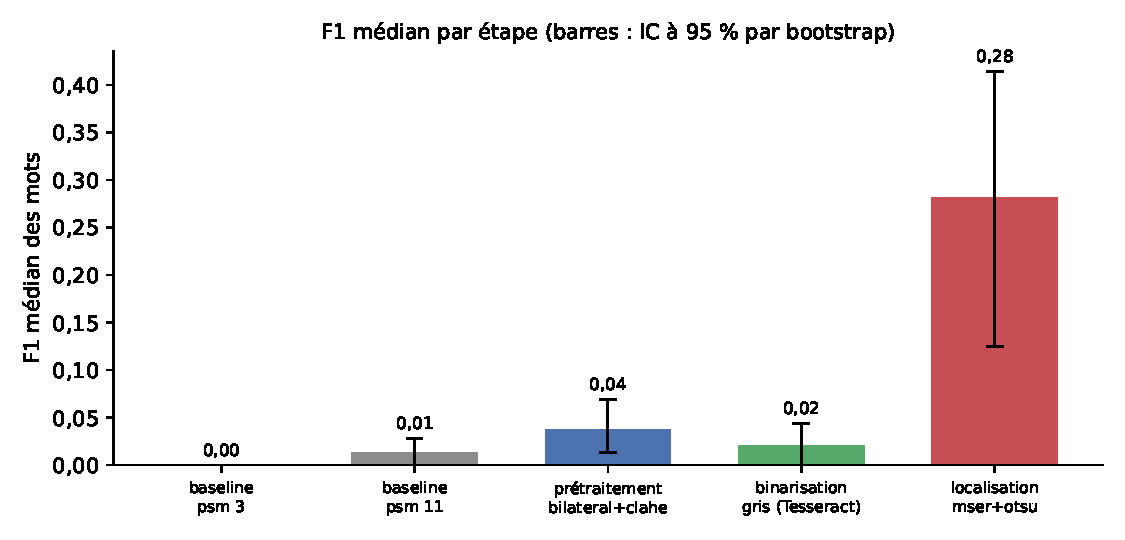
\includegraphics[width=\linewidth]{progression.pdf}\end{subfigure}\hfill
\begin{subfigure}{0.41\linewidth}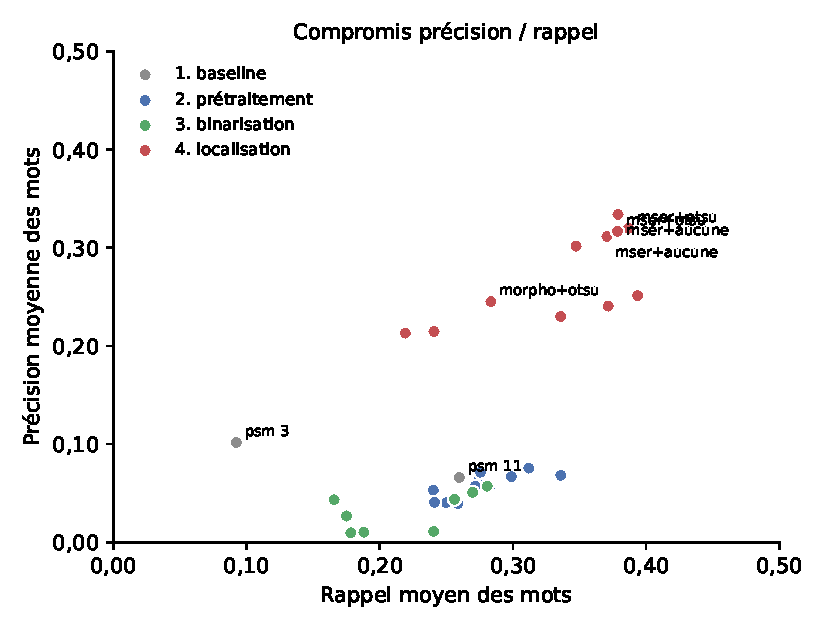
\includegraphics[width=\linewidth]{precision_rappel.pdf}\end{subfigure}
\caption{Gauche : F1 médian des mots et intervalle de confiance à 95\,\% par étape. Droite : précision et rappel moyens de toutes les configurations ; la localisation déplace les configurations vers le haut et la droite.}
\label{fig:progression}
\end{figure}

\subsection{Résultats par catégorie}
Le tableau~\ref{tab:categories} détaille les résultats par catégorie. Les plaques et les panneaux, qui représentent 42 images sur 50, progressent nettement en précision comme en rappel. Les affiches font exception : la précision augmente, mais le rappel médian baisse. Leurs polices décoratives, enseignes lumineuses et textes inclinés échappent au détecteur, alors que la baseline en lisait une partie au milieu de nombreuses inventions. Les numéros (3 images seulement) restent hors de portée. Ces deux petites catégories ne permettent pas de conclusion ferme, mais elles indiquent où la localisation doit progresser.

\tableauOuNote{tableau_categories.tex}{Tableau par catégorie non encore généré.}

\subsection{Analyse des échecs}\label{sec:echecs}
Huit images restent à $F_1=0$ quelle que soit la configuration, y compris après les corrections de la version~2. Pour chacune, nous avons fourni à Tesseract la zone de texte recadrée à la main, ce qui permet de distinguer deux types d'échec : si Tesseract lit la zone recadrée, l'échec vient de la \emph{localisation} et peut être corrigé ; sinon, il vient de la \emph{reconnaissance}, et dépasse ce que permettent les outils imposés (tableau~\ref{tab:echecs}, figure~\ref{fig:echecs}).

\begin{table}[htbp]
\centering\small
\begin{tabular}{p{2.2cm}p{5.4cm}p{2.4cm}p{4.2cm}}
\toprule
Image & Cause & Type & Correction \\
\midrule
plaques\_016 & lettres blanches sur plaque dorée : pas de contraste de luminance & localisation & canal $b$ de Lab (figure~\ref{fig:couleur}) \\
plaques\_036 & petit panneau à contre-jour & localisation & recadré et agrandi 3 fois, Tesseract lit \og LANFOUD\fg \\
plaques\_032 & écriture arabe (STOP) : le détecteur suppose des lettres latines séparées & localisation & avec la zone et la langue arabe, Tesseract lit le mot \\
plaques\_024 & lettres gravées, visibles seulement par leurs ombres & les deux & canal CLAHE : \og PALATINE\fg{} lu \\
plaques\_041 & arabe peint à la main & reconnaissance & aucune \\
affiches\_007 & néon de nuit, lettres creuses et cursives & reconnaissance & seul \og NEXOTTEL\fg{} est lisible \\
plaques\_043 & texte de 6 à 8~px de haut & reconnaissance & illisible même agrandi 5 fois \\
plaques\_033 & texte lu correctement (\og AMBASSADE DE FRANCE\fg) mais absent de la vérité terrain & annotation & compléter l'annotation \\
\bottomrule
\end{tabular}
\caption{Diagnostic des images en échec.}
\label{tab:echecs}
\end{table}

\begin{figure}[htbp]
\centering
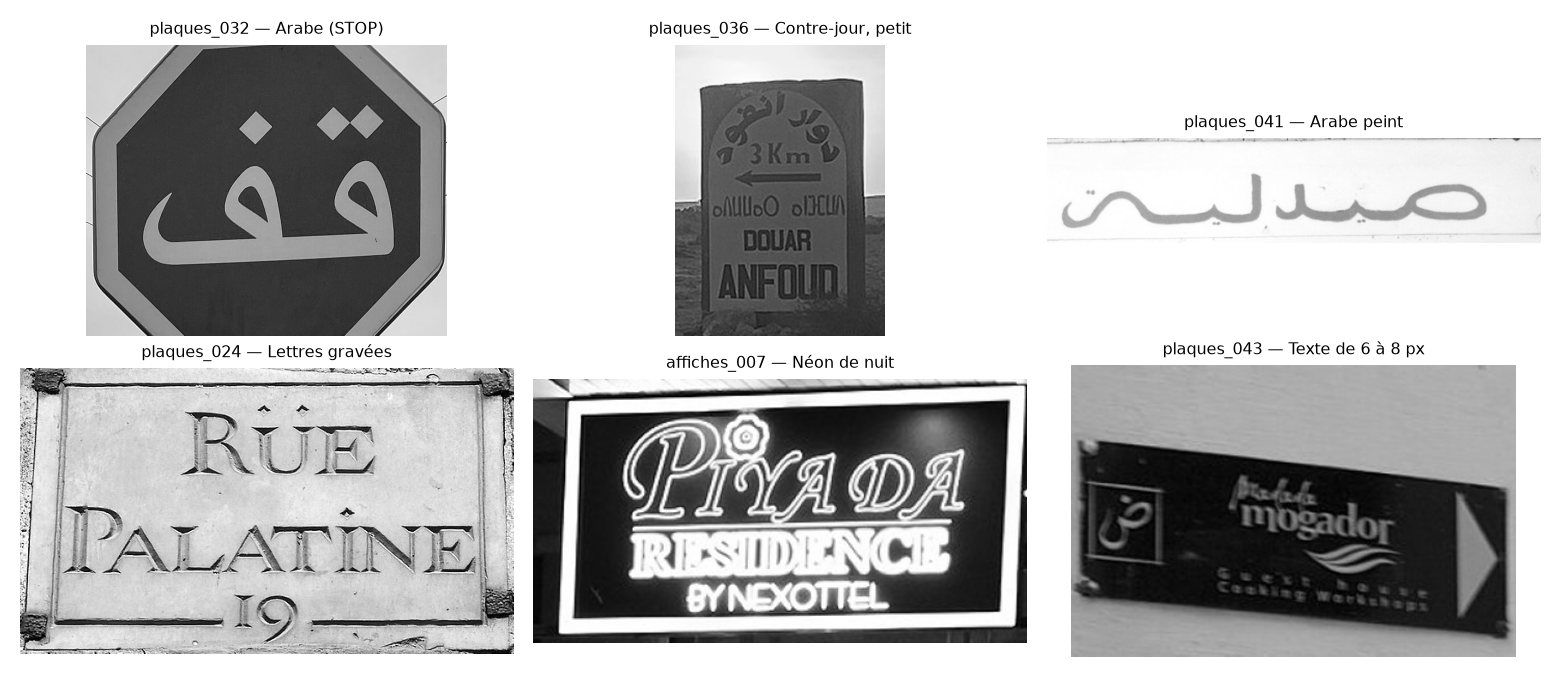
\includegraphics[width=\linewidth]{echecs.png}
\caption{Zones de texte des images en échec, recadrées à la main.}
\label{fig:echecs}
\end{figure}

Trois corrections en ont été tirées. La hauteur minimale d'une ligne a été abaissée de 0,8\,\% à 0,5\,\% de la hauteur de l'image, ce qui permet par exemple de trouver \og RANDAN\fg{} sur un poteau de signalisation. Un plafond de 40 zones lues par image limite le temps de calcul. Les canaux couleur et CLAHE, enfin, sont proposés en option : sur 13 images de test, ils font passer le F1 moyen de 0,226 à 0,278, mais doublent le temps de calcul et créent de fausses zones sur certaines images. Ils n'ont pas été évalués sur la base complète et restent donc désactivés par défaut ; c'est la première expérience à mener pour prolonger ce travail.

\subsection{Temps de calcul}
Sur un processeur de bureau, la configuration finale demande en moyenne 5,5~s par image (sans canaux supplémentaires), dont l'essentiel est passé dans les appels à Tesseract, un par zone. Sans plafond (première version), la moyenne était de 8,3~s et les pires cas atteignaient 49~s sur des scènes de feuillage où plus de 90 zones étaient envoyées à Tesseract ; le plafond de 40 zones ramène le pire cas à 19~s. La baseline prend environ 4~s par image.

% -----------------------------------------------------------------------------
\section{Discussion}
% -----------------------------------------------------------------------------

\paragraph{Ce que montrent les résultats.} Dans une scène urbaine, la difficulté principale de l'OCR n'est pas la qualité de l'image mais la séparation du texte et du reste. Les traitements classiques d'amélioration (débruitage, contraste, binarisation) restent utiles, mais \emph{à l'intérieur} des zones de texte, une fois celles-ci localisées. La morphologie mathématique et la segmentation en composantes connexes jouent un rôle central dans cette localisation : retrait des traits, fermeture, vérification par la régularité des caractères, profils de projection.

\paragraph{Limites.} Le F1 médian final reste modeste en valeur absolue : environ un mot sur trois est retrouvé, et environ un mot lu sur trois est juste. Les causes identifiées sont l'écriture arabe, très présente au Maroc, les lettres gravées ou en relief, l'éclairage artificiel nocturne, le texte de très petite taille et les polices décoratives. La base reste petite, surtout pour les numéros et les affiches, et les règles d'annotation influencent les scores.

\paragraph{Perspectives.}
\begin{itemize}
\item \textbf{Écriture arabe} : adapter la vérification des lignes aux écritures cursives (composantes larges, une par mot) et activer la langue \texttt{ara} de Tesseract sur les zones concernées.
\item \textbf{Détecteurs appris} : les détecteurs de texte par réseaux de neurones (EAST, CRAFT, DBNet) sont l'état de l'art pour les scènes ; ils sortent du cadre des outils imposés, mais le module de localisation est conçu pour être remplacé sans toucher au reste du pipeline.
\item \textbf{Restitution vocale} : brancher une synthèse vocale sur le texte brut produit par la restitution.
\item \textbf{Temps réel} : paralléliser les appels à Tesseract et ne lire que les zones proches du centre de l'image, là où l'utilisateur vise.
\end{itemize}

% -----------------------------------------------------------------------------
\section{Conclusion}
% -----------------------------------------------------------------------------
Nous avons réalisé un pipeline complet, de la photographie à la restitution accessible, en mesurant l'apport de chaque étape. La baseline montre que Tesseract seul est inutilisable sur des scènes urbaines (F1 médian de \baseFmed). La localisation du texte par MSER, la vérification par segmentation des caractères et la lecture zone par zone portent ce score à \finFmed{}, soit environ \facteurF{} fois plus, avec une amélioration significative sur \finMieux{} images sur \nbImages. L'analyse des échecs délimite clairement ce que permettent les techniques classiques et indique les pistes prioritaires : la prise en charge de l'arabe et une détection plus robuste aux conditions d'éclairage.

% -----------------------------------------------------------------------------
\appendix
\section{Utilisation}
% -----------------------------------------------------------------------------
\begin{verbatim}
uv sync                                       # installer l'environnement
uv run scripts/lire_image.py photo.jpg --carte c.png
uv run scripts/baseline_tesseract.py          # baseline
uv run scripts/etape2_pretraitement.py --ocr  # prétraitement
uv run scripts/etape3_binarisation.py --ocr   # binarisation
uv run scripts/etape4_localisation.py         # localisation + OCR par région
uv run scripts/benchmark.py                   # tableaux et figures du rapport
cd docs/rapport && latexmk -pdf rapport.tex   # recompiler
\end{verbatim}
Avec Docker (Tesseract inclus) : \texttt{docker compose run --rm ocr scripts/lire\_image.py data/images/...}

% -----------------------------------------------------------------------------
\begin{thebibliography}{99}
\small
\bibitem{otsu} N.~Otsu. A threshold selection method from gray-level histograms. \emph{IEEE Trans. Systems, Man, and Cybernetics}, 9(1):62--66, 1979.
\bibitem{triangle} G.~W.~Zack, W.~E.~Rogers, S.~A.~Latt. Automatic measurement of sister chromatid exchange frequency. \emph{J. Histochemistry \& Cytochemistry}, 25(7):741--753, 1977.
\bibitem{niblack} W.~Niblack. \emph{An Introduction to Digital Image Processing}. Prentice Hall, 1986.
\bibitem{sauvola} J.~Sauvola, M.~Pietikäinen. Adaptive document image binarization. \emph{Pattern Recognition}, 33(2):225--236, 2000.
\bibitem{bilateral} C.~Tomasi, R.~Manduchi. Bilateral filtering for gray and color images. \emph{ICCV}, 1998.
\bibitem{nlm} A.~Buades, B.~Coll, J.-M.~Morel. A non-local algorithm for image denoising. \emph{CVPR}, 2005.
\bibitem{clahe} K.~Zuiderveld. Contrast limited adaptive histogram equalization. In \emph{Graphics Gems IV}, Academic Press, 1994.
\bibitem{immerkaer} J.~Immerkær. Fast noise variance estimation. \emph{Computer Vision and Image Understanding}, 64(2):300--302, 1996.
\bibitem{ssim} Z.~Wang, A.~C.~Bovik, H.~R.~Sheikh, E.~P.~Simoncelli. Image quality assessment: from error visibility to structural similarity. \emph{IEEE Trans. Image Processing}, 13(4):600--612, 2004.
\bibitem{mser} J.~Matas, O.~Chum, M.~Urban, T.~Pajdla. Robust wide baseline stereo from maximally stable extremal regions. \emph{BMVC}, 2002.
\bibitem{neumann} L.~Neumann, J.~Matas. Real-time scene text localization and recognition. \emph{CVPR}, 2012.
\bibitem{tesseract} R.~Smith. An overview of the Tesseract OCR engine. \emph{ICDAR}, 2007.
\end{thebibliography}

\end{document}
